\chapter{Homotopy Theory}

All spaces under consideration are connected.

\section{Mapping Cylinder and Mapping Path Space}
    In the homotopy theory, every map $f: A \to B$ 
    can be viewed as an inclusion or a fibration up to homotopy. 

    \textbf{Inclusion}:
    The mapping cylinder of $f$ is defined as
    \begin{equation*}
        M_f = (A\times I)\sqcup B\big/(a,1)\sim f(a).
    \end{equation*}
    
    We have an inclusion $j: A\hookrightarrow M_f$ defined by 
    \begin{align*}
        j:A&\hookrightarrow M_f \\
        a &\mapsto(a,0),
    \end{align*}
    an inclusion $i: B\hookrightarrow M_f$ defined by
    \begin{align*}
        i:B&\hookrightarrow M_f \\
        b &\mapsto b,
    \end{align*}
    and a retraction $r: M_f \to B$ defined by
    \begin{align*}
        r:M_f&\to B \\
        (a,t) &\mapsto f(a); \\
        b &\mapsto b.
    \end{align*}
    Note that $r\circ i = \id_B$ and $i\circ r \simeq \id_{M_f}$ 
    through the homotopy
    \begin{align*}
        H: M_f &\times I \to M_f \\
        ((a,t),s) &\mapsto (a,(1-s)t+s); \\
        (b,s) &\mapsto b. 
    \end{align*}
    Geometrically, the homotopy $H$ can be viewed as 
    the process of continuously collapsing 
    the cylinder $A\times I$ in $M_f$ down onto 
    the image of $f$ in $B$.

    Since $r\circ j = f$, we have a commutative diagram
    \begin{center}
        \begin{tikzcd}
         & M_f \arrow[rd, "\simeq"] &   \\
        A \arrow[rr, "f"] \arrow[ru, "j", hook] & & B
        \end{tikzcd}
    \end{center}
    in this sense, $f$ is homotopic to the inclusion $j$.

    \textbf{Fibration}:
    The mapping path space of $f$ is defined as
    \begin{equation*}
        P_f =\left\{(a,\gamma) \in A\times\mathcal{P}(B)\,\Big|\,
        \gamma(1) = f(a)\right\}.
    \end{equation*}
    where
    \begin{equation*}
        \mathcal{P}(B) = \left\{\gamma: I\to B\right\}
    \end{equation*}
    is the path space of $B$ having arbitrary starting point 
    and ending point.
    
    We have a fibration $p: P_f \to B$ defined by
    \begin{align*}
        p: P_f &\to B \\
        (a,\gamma) &\mapsto \gamma(0).
    \end{align*}
    The fiber of $p$ over a point $b\in B$ is given by
    \begin{equation*}
        \Omega_{b}^{A}:=p^{-1}(b)
            =\left\{(a,\gamma)\in A\times\mathcal{P}(B)\,\Bigg|\,
            \begin{array}{l}
                \gamma(0)=b \\
                \gamma(1)=f(a)
            \end{array}
            \right\}.
    \end{equation*}
    We have an inclusion $j: A\hookrightarrow P_f$ defined by
    \begin{align*}
        i:A&\hookrightarrow P_f \\
        a &\mapsto(a,c_{f(a)}),
    \end{align*}
    where $c_{f(a)}$ is the constant path at $f(a)$,
    and a retraction $r: P_f \to A$ defined by
    \begin{align*}
        r: P_f &\to A \\
        (a,\gamma) &\mapsto a.
    \end{align*}
    Note that $r\circ i = \id_A$ and $i\circ r \simeq \id_{P_f}$
    through the homotopy
    \begin{align*}
        H: P_f &\times I \to P_f \\
        ((a,\gamma),s) &\mapsto (a,\tilde{\gamma}_s).
    \end{align*}
    where $\tilde{\gamma}_s(t)=\gamma(s+(1-s)t)$ for $t\in I$ is 
    a path in $B$ that starts at $\gamma(s)$ and ends at $\gamma(1)$.
    Geometrically, the homotopy $H$ can be viewed as 
    the process of continuously collapsing 
    the path $\gamma$ in $P_f$ down onto 
    the constant path $c_{f(a)}$.

    Since $r\circ j = f$, we have a commutative diagram
    \begin{center}
        \begin{tikzcd}
         & P_f \arrow[rd, "p", two heads] &   \\
        A \arrow[rr, "f"] \arrow[ru, "\simeq"] & & B
        \end{tikzcd}
    \end{center}
    in this sense, $f$ is homotopic to the fibration $p$. 

    \begin{remark}
        The mapping cylinder can be constructed as a pushout of the diagram
        \begin{center}
            \begin{tikzcd}
                A \arrow[r, "\iota_0", hook] \arrow[d, "f"'] & A\times I \arrow[d] \\
                B \arrow[r] & M_f
                \arrow[ul, phantom, very near start, "\ulcorner"]
            \end{tikzcd}
        \end{center}
        where $\iota_0: A\hookrightarrow A\times I$ is the inclusion map
        defined by $\iota_0(a) = (a,0)$.

        The mapping path space can be constructed as a pullback of 
        the diagram
        \begin{center}
            \begin{tikzcd}
                P_f \arrow[dr, phantom, very near start, "\lrcorner"] 
                \arrow[r] \arrow[d] & A \arrow[d, "f"]\\
                \mathcal{P}(B) \arrow[r, "\mathrm{ev}", two heads] & B 
            \end{tikzcd}
        \end{center}
        where $\mathrm{ev}: \mathcal{P}(B) \to B$ 
        is the evaluation map defined by 
        $\mathrm{{ev}}(\gamma) = \gamma(0)$.
    \end{remark}

    \subsection{Postnikov tower and Whitehead tower}
    We know that the homotopy type of a space $X$ can be captured 
    by its homotopy groups $\pi_q=\pi_q(X)$. In homotopy theory, 
    the simplest spaces are the Eilenberg-MacLane spaces $K(A,n)$. 
    So there is a natural question:
    \begin{center}
        \fbox{\parbox{0.8\linewidth}{
            \centering
            Can we decompose $X$ as a "product" of a sequence of 
            Eilenberg-MacLane spaces?
        }}
    \end{center}
    The directly product of Eilenberg-MacLane spaces is not enough 
    to capture the homotopy type of $X$ in general, i.e.,
    \begin{equation*}
        X \not\simeq \prod_{q}K(\pi_q(X),q).
    \end{equation*} 
    So we need to introduce a more general construction,
    the Postnikov tower, and the Whitehead tower.
    \begin{definition}[Postnikov tower]
        Given a CW complex $X$ and an integer $n$, the Postnikov tower of $X$ is a sequence 
        of fibrations
        \begin{center}
            \begin{tikzcd}
                                                        % & \vdots \arrow[d] &                                     \\
            {K(\pi_n,n)} \arrow[r]                      & Y_n \arrow[d]    &                                     \\
                                                        & \vdots \arrow[d] &                                     \\
            {K(\pi_2,2)} \arrow[r]                      & Y_2 \arrow[d]    &                                     \\
            {K(\pi_1,1)} \arrow[r, Rightarrow, no head] & Y_1              & X \arrow[l] \arrow[lu] \arrow[luuu]
            \end{tikzcd}
        \end{center}
        satisfying the following properties:
        \begin{itemize}
            \item 
            \begin{equation*}
                \pi_k(Y_q) = 
                \begin{cases}
                    0 &, k>q; \\
                    \pi_k(X) &, k\leq q.
                \end{cases}
            \end{equation*}
            \item the fibration $Y_q\to Y_{q-1}$ has fiber $K(\pi_q,q)$ 
            and commutes with the maps $X\to Y_q$; 
            \item the map $X\to Y_q$ induces isomorphisms
            \begin{equation*}
                \pi_k(X) \xrightarrow{\cong} \pi_k(Y_q), \quad k\leq q.
            \end{equation*}
        \end{itemize}
    \end{definition}
    \textbf{Construction:}
    The space $Y_q$ is the space obtained from $X$ by truncating 
    its homotopy groups above degree $q$. 

    \textbf{Step 1: Construct $Y_n$ from $X$}
    
    To construct $Y_n$, we have to 
    kill the homotopy groups $\pi_k(X)$ for $k>n$. 
    The method is attaching cells.
    To be more precise, if $\alpha: S^{n+1} \to X$ is a generator of 
    $\pi_{n+1}(X)$, we can attach a cell $e^{n+2}$ to $X$, i.e.,
    \begin{equation*}
        X \cup_{\alpha} e^{n+2} = X \sqcup e^{n+2} \big/ x\sim \alpha(x)
    \end{equation*}
    to kill the generator $\alpha$ in $\pi_{n+1}(X)$,
    Rrepeat this process for all generators of $\pi_{n+1}(X)$, we get $X_1$. 
    Note that this process does not change the homotopy groups
    $\pi_k(X)$ for $k\leq n$. 
    Then we can repeat this process for $X_1$ to get $Y_n$.
    \begin{equation*}
        Y_n = X \cup_{\alpha} e^{n+2} \cup \cdots
    \end{equation*}
    we have a natural inclusion $X \hookrightarrow Y_n$.

    \textbf{Step 2: Inductively construct $Y_{q-1}$ from $Y_q$}

    To construct $Y_{q-1}$ from $Y_q$, we have to kill $\pi_q(Y_q)$. 
    The method is similar to the previous step, i.e., attaching cells.
    \begin{equation*}
        Y_{q-1} = Y_q \cup e^{q+1} \cup \cdots
    \end{equation*}
    therefore we have a natural inclusion $Y_q \hookrightarrow Y_{q-1}$. 
    It can be viewed as a fibration 
    \begin{center}
        \begin{tikzcd}
            F_q \arrow[r] & Y_q \arrow[d] \\
            & Y_{q-1}
        \end{tikzcd}
    \end{center}

    \textbf{Step 3: Check $F_q$ is $K(\pi_q,q)$}

    The fibration induces a long exact sequence of homotopy groups
    \begin{equation*}
        \cdots \to \pi_{k+1}(Y_q) \to \pi_{k+1}(Y_{q-1}) 
        \to \pi_k(F_q) \to \pi_k(Y_q) \to \pi_k(Y_{q-1}) \to \cdots
    \end{equation*}
    \begin{itemize}
        \item $k\geq q+1$: $\pi_{k+1}(Y_{q-1}) = \pi_{k}(Y_q) = 0$,
        so $\pi_k(F_q) = 0$. 
        \item $k=q$: $\pi_{q+1}(Y_{q-1}) = \pi_{q}(Y_{q-1}) = 0$,
        so $\pi_q(F_q) = \pi_q(Y_q) = \pi_q(X)$.
        \item $k=q-1$: $\pi_{q}(Y_{q-1}) = 0$, 
        $\pi_{q-1}(Y_q) \cong \pi_{q-1}(X)$, so $\pi_{q-1}(F_q) = 0$.
        \item $k\leq q-2$: $\pi_{k+1}(Y_{q}) \cong \pi_{k+1}(Y_{q-1})$,
        so $\pi_k(F_q) = 0$.
    \end{itemize}
    Therefore, we have
    \begin{equation*}
        \pi_k(F_q) = 
        \begin{cases}
            \pi_q(X) &, k=q; \\
            0 &, k\neq q.
        \end{cases}
    \end{equation*}
    So $F_q\simeq K(\pi_q,q)$. 
    \qed

    \begin{definition}[Whitehead tower]
        Given a CW complex $X$, the Whitehead tower of $X$ is a sequence
        of fibrations
        \begin{center}
            \begin{tikzcd}
                                        & \vdots \arrow[d]  \\
            {K(\pi_n,n-1)} \arrow[r]     & X_n \arrow[d]     \\
            {K(\pi_{n-1},n-2)} \arrow[r] & X_{n-1} \arrow[d] \\
                                        & \vdots \arrow[d]  \\
            {K(\pi_1,0)} \arrow[r]       & X_1 \arrow[d]     \\
                                        & X                
            \end{tikzcd}
        \end{center}
        satisfying the following properties:
        \begin{itemize}
            \item 
            \begin{equation*}
                \pi_k(X_n) = 
                \begin{cases}
                    0 &, k\leq n; \\
                    \pi_k(X) &, k>n.
                \end{cases}
            \end{equation*}
            \item the fibration $X_n\to X_{n-1}$ has fiber $K(\pi_n,n-1)$.
        \end{itemize}
    \end{definition}

    \textbf{Construction:}
    The space $X_1$ is the universal cover of $X$ in the homotopy sense. 
    The space $X_n$ is the generalization of $X_1$ to higher dimensions. 
    
    \textbf{Step 1: Construct $X_1$ from $X$}
    
    To construct $X_1$, we have to kill $\pi_1(X)$. 
    First kill the higher homotopy groups of $X$ to get
    \begin{equation*}
        Y_1 = X \cup e^3 \cup \cdots = K(\pi_1(X),1)
    \end{equation*}
    $X$ is naturally included in $Y_1$. We define 
    \begin{equation*}
        X_1 = \Omega_{*}^{X} = \left\{(x,\gamma) \in X\times\mathcal{P}(Y_1)
        \,\Bigg|\, 
        \begin{aligned}
            \gamma(0) &= * \\
            \gamma(1) &= x
        \end{aligned}
        \right\}.
    \end{equation*} 
    The projection $p: X_1 \to X$ is a fibration with fiber
    \begin{equation*}
        p^{-1}(*)=\Omega Y_1 = K(\pi_1,0).
    \end{equation*}
    We can show that 
    \begin{align*}
        \pi_k(X_1) &= 
        \begin{cases}
            \pi_k(X) &, k\geq 2; \\
            0 &, k\leq 1. 
        \end{cases}
    \end{align*}
    So $X_1$ is the universal cover of $X$ in the homotopy sense.

    \textbf{Step 2: Inductively construct $X_n$ from $X_{n-1}$}

    Firstly, kill the higher homotopy groups of $X_{n-1}$ to get
    \begin{equation*}
        Y_n = X_{n-1} \cup e^{n+2} \cup \cdots = K(\pi_n,n).
    \end{equation*}
    Then we can repeat the process for $X_n$ to get
    \begin{equation*}
        X_n = \Omega_{*}^{X_{n-1}}
    \end{equation*}
    The projection $p: X_n \to X_{n-1}$ gives a fibration 
    \begin{center}
        \begin{tikzcd}
            K(\pi_n,n-1)=\Omega Y_n \arrow[r] & X_n \arrow[d] \\
            & X_{n-1}
        \end{tikzcd}
    \end{center}

    \textbf{Step 3: Check $\pi_k(X_n)$}
    
    The fibration induces a long exact sequence of homotopy groups
    \begin{equation*}
        \cdots \to \pi_{k+1}(X_{n-1}) \xrightarrow{\delta} \pi_k(\Omega Y_n) 
        \to \pi_k(X_n) \to \pi_k(X_{n-1}) \xrightarrow{\delta} \pi_{k-1}(\Omega Y_n) \to \cdots
    \end{equation*}
    \begin{itemize}
        \item $k\geq n+1$: $\pi_{k}(\Omega Y_n) = \pi_{k-1}(\Omega Y_n) = 0$. 
        So $\pi_k(X_n) \cong \pi_k(X_{n-1}) = \pi_k(X)$.
        \item $k=n,n-1$: 
        \begin{equation*}
        \hspace*{-2em}
        \pi_{n}(\Omega Y_n) \to \pi_{n}(X_n) \to \pi_{n}(X_{n-1}) 
        \xrightarrow{\delta} \pi_{n-1}(\Omega Y_n) \to \pi_{n-1}(X_n) 
        \to \pi_{n-1}(X_{n-1})
        \end{equation*}
        \textcolor{red}{
        The connecting homomorphism 
        $\delta: \pi_{n}(X_{n-1}) \to \pi_{n-1}(\Omega Y_n)$ 
        is an isomorphism,} 
        $\pi_n(\Omega Y_n) = \pi_{n+1}(Y_n) = 0$,
        $\pi_{n-1}(X_{n-1}) = 0$. So $\pi_n(X_n) = 0$. 
        \item $k\leq n-2$: $\pi_k(\Omega Y_n) = \pi_k(X_{n-1}) = 0$. 
        So $\pi_k(X_n) = 0$. 

    \end{itemize}
    Therefore, we have 
    \begin{equation*}
        \pi_k(X_n) = 
        \begin{cases}
            \pi_k(X) &, k\geq n+1; \\
            0 &, k\leq n. 
        \end{cases}
    \end{equation*} 
    
    \textbf{Why $\delta$ is an isomorphism?}

    The connecting homomorphism $\delta$ is defined as follows:
    \begin{align*}
        \delta: \pi_{n}(X_{n-1}) &\to \pi_{n-1}(\Omega Y_n) \\
        [\alpha] &\mapsto [\tilde{\alpha}],
    \end{align*}
    where $\alpha: (I^n,\partial I^n) \to (X_{n-1},*)$ represents $[\alpha]$. 
    $\tilde{\alpha}: (I^{n-1},\partial I^{n-1}) \to (\Omega Y_n,c_*)$ 
    is defined by 
    \begin{equation*}
        \tilde{\alpha}(s)(t) = \alpha(s,t), 
        \quad (s,t)\in I^{n-1}\times I = I^n. 
    \end{equation*}
    This is essentially treating the last coordinate of $\alpha$ 
    as the time parameter of the path. Note that the connecting homomorphism 
    \begin{align*}
        \delta': \pi_{n}(Y_n) &\xrightarrow{\cong} \pi_{n-1}(\Omega Y_n) \\
        [\alpha] &\mapsto [\tilde{\alpha}],
    \end{align*}
    is defined in the same way. $\delta$ is excatly the composition of 
    two isomorphisms:
    \begin{center}
        \begin{tikzcd}
        \pi_{n}(X_n) \arrow[r, "\iota^*"', "\cong"] \arrow[rr, "\delta", bend left] 
        & \pi_n(Y_n) \arrow[r, "\delta'"',"\cong"] & \pi_{n-1}(\Omega Y_n)
        \end{tikzcd}
    \end{center}
    Therefore, $\delta$ is an isomorphism.
    \qed

    \begin{remark}
        Postnikov tower 将空间 $X$ 从小空间一点一点拼装起来; 
        Whitehead tower 则是将空间 $X$ 从基本群开始逐步解开. 
        
        在Postnikov tower 中, 每一项 $Y_n$ 具有特殊的胞腔分解
        \begin{equation*}
            Y_n = X \cup e^{n+2} \cup \cdots
        \end{equation*}
        所以我们能得到 $Y_n$ 的同调群信息.
        
        在Whitehead tower 中, 每一项 $X_n$ 都是 $n$-连通空间, 
        所以我们能得到 $X_n$ 的同调群信息.
    \end{remark}

    \subsection{The rational homotopy groups of spheres}
    The rational homotopy groups of spheres are given by the following theorem:
    \begin{theorem}[Sere theorem]
        If $n$ is odd, then
        \begin{equation*}
            \pi_q(S^n)\otimes\mathbb{Q} =
            \begin{cases}
                \mathbb{Q} &, q=0, n; \\
                0 &, \text{otherwise}.
            \end{cases}
        \end{equation*}
        If $n$ is even, then
        \begin{equation*}
            \pi_q(S^n)\otimes\mathbb{Q} =
            \begin{cases}
                \mathbb{Q} &, q=0, n, 2n-1; \\
                0 &, \text{otherwise}.
            \end{cases}
        \end{equation*}
    \end{theorem} 
    Before proving this theorem, we need two lemmas. 
    \begin{lemma}
        All $\pi_q(S^n)$ are finitely generated abelian groups.
    \end{lemma}
    The proof of this lemma is based on Serre's 
    $\mathscr{C}$-class. We skip the details here. 
    \begin{lemma}\label{coho-of-EMspace}\hfill
        \begin{itemize}
            \item For any finite abelian group $A$, $H^*(K(A,n);\mathbb{Q})=0$.
            \item The cohomology ring $H^*(K(\mbb{Z},n);\mbb{Q})$ is free on one 
            generator of degree $n$, i.e., 
            \begin{equation*}
                H^*(K(\mbb{Z},n);\mbb{Q}) =
                \begin{cases}
                    \Lambda(x), \dim x=n,\quad n \rm{\ is\ odd }; \\
                    \mbb{Q}[x], \dim x=n,\quad n \rm{\ is\ even }.
                \end{cases}
            \end{equation*}
        \end{itemize}
    \end{lemma}
    \begin{proof}
        For $n=1$, $K(\mbb{Z},1)\simeq S^1$,
        so $H^*(K(\mbb{Z},1);\mbb{Q})\cong\Lambda(x),\;\dim x=1$.

        For $n=2$, $K(\mbb{Z},2)\simeq \mbb{C}P^\infty$,
        so $H^*(K(\mbb{Z},2);\mbb{Q})\cong\mbb{Q}[x],\;\dim x=2$.

        For $n\geq 3$, we use the fibration 
        \begin{center}
            \begin{tikzcd}
            {K(\mathbb{Z},2)} \arrow[r] & {\mathcal{P}K(\mathbb{Z},3)} \arrow[d] \\
                                        & {K(\mathbb{Z},3)}                     
            \end{tikzcd}
        \end{center}
        Its associated Serre spectral sequence has $E_2$-term
        \begin{sseqdata}[ name = KZ3, xscale = 0.7 , yscale = 0.6, 
        cohomological Serre grading ,classes = {draw = none}]
        \begin{scope}[background]
        \node at (\xmax/2,\ymax+1.2) {\textup{Page \page}};
        \node at (\xmax/2,-3) {H^*(K(\mbb{Z},3))};
        \node at (-3,\ymax/2) {H^*(\mbb{C}P^\infty)};
        \end{scope}
        \class["\mbb{Q}"](0,0)
        \class["x"](0,2)
        \class["x^2"](0,4)
        \class["a"](3,0)
        \class["ax"](3,2)
        \class["ax^2"](3,4)
        \class["\vdots"](0,6)
        \class["\vdots"](3,6)
        \d["\simeq"']3(0,2)
        \d["\cdot2"']3(0,4)
        \d["\cdot3"']3(0,6)
        \end{sseqdata}
        \begin{center}
            \printpage[ name = KZ3, page = 3 ]
        \end{center}
        To cancel $x$, we have to set $d_3 x = a$ to be an isomorphism. 
        The above diffrential map is given by product structure. Since 
        we are working with rational coefficients, they are all isomorphisms.
        So we have $E_4 = E_\infty$. Therefore, we have
        \begin{equation*}
            H^*(K(\mbb{Z},3);\mbb{Q}) = \Lambda(x),\; \dim x = 3.
        \end{equation*}
        
        For $n\geq 4$, we can use the fibration
        \begin{center}
            \begin{tikzcd}
            {K(\mathbb{Z},3)} \arrow[r] & {\mathcal{P}K(\mathbb{Z},4)} \arrow[d] \\
                                        & {K(\mathbb{Z},4)}                     
            \end{tikzcd}
        \end{center}
        Its associated Serre spectral sequence has $E_2$-term
        \begin{sseqdata}[ name = KZ4, xscale = 0.5 , yscale = 0.5, 
        cohomological Serre grading ,classes = {draw = none}]
        \begin{scope}[background]
        \node at (\xmax/2,\ymax+1.2) {\textup{Page \page}};
        \node at (\xmax/2,-3) {H^*(K(\mbb{Z},4))};
        \node at (-4.7,\ymax/2) {H^*(K(\mbb{Z},3))};
        \end{scope}
        \class["\mbb{Q}"](0,0)
        \class["x"](0,3)
        \class["a"](4,0)
        \class["ax"](4,3)
        \class["a^2"](8,0)
        \class["a^2x"](8,3)
        \class["\cdots"](12,0)
        \class["\cdots"](12,3)
        \d["\sim"']4(0,3)
        \d["\cdot2"']4(4,3)
        \d["\cdot3"']4(8,3)
        \end{sseqdata}
        \printpage[ name = KZ4, page = 4 ] \\
        Therefore, we have
        \begin{equation*}
            H^*(K(\mbb{Z},4);\mbb{Q}) = \mbb{Q}[x],\; \dim x = 4.
        \end{equation*}
        By induction, we can get the result for all $n\geq 5$.
    \end{proof}

    Now we can prove the Sere theorem. There are two ways to prove it,
    one is using the Postnikov tower, 
    the other is using the Whitehead tower.
    \begin{proof}[Proof of Sere theorem using Postnikov tower]
        Since $S^n$ is $n$-connected, we have the Postnikov tower
        \begin{center}
            \begin{tikzcd}
                & \vdots \arrow[d] \\
                K(\pi_{n+2},n+2) \arrow[r] & Y_{n+2} \arrow[d] \\
                K(\pi_{n+1},n+1) \arrow[r] & Y_{n+1} \arrow[d] \\
                & K(\mbb{Z},n)
            \end{tikzcd}
        \end{center}
        \textcolor{red}{
        By the construction of the Postnikov tower, we have
        \begin{equation*}
            Y_q = S^n \cup e^{q+2} \cup \cdots,\quad q\geq n+1.
        \end{equation*}
        Hence the cohomology groups of $Y_q$ satisfies
        \begin{equation*}
            H^{q}(Y_q;\mbb{Q}) = H^{q+1}(Y_q;\mbb{Q}) = 0.
        \end{equation*}
        }

        \noindent If n is odd:
        
        \noindent$\circ\;\dim = n+1$: 
        The fibration $Y_{n+1} \to K(\mbb{Z},n)$ has spectral sequence

        \begin{sseqdata}[ name = SereOddPostnikov1, 
        xscale = 1 , yscale = 1, 
        no x ticks, no y ticks, 
        cohomological Serre grading, classes = {draw = none}]
        \begin{scope}[background]
        \node at (\xmax/2,-2) {H^*(K(\mbb{Z},n))};
        \node[rotate = 90] at (-2.2,\ymax/2) {H^*(K(\pi_{n+1},n+1))};
        \node at (0,\ymin-1) {0};
        \node at (4,\ymin-1) {\protect\vphantom{2}n};
        \node at (6,\ymin-1) {\protect\vphantom{2}n+2};
        % \node at (5,\ymin-1) {\protect\vphantom{2}n+1};
        \node at (\xmin-1,0) {0};
        \node at (\xmin-1.3,5) {\protect\vphantom{2}n+1};
        \end{scope}
        \class["\mbb{Q}"](0,0)
        \class["\mbb{Q}"](4,0)
        \class["\pi_{n+1}"](0,5)
        \class["0"](5,0)
        \class["0"](6,0)
        \class(7,0)
        \class["*"](0,6)
        \class["*"](0,7)
        \d6(0,5)
        \circleclasses[rounded rectangle](5,0)(0,5)
        \end{sseqdata}
        \begin{center}
            \printpage[ name = SereOddPostnikov1, page = 6 ]
        \end{center}
        Since $K(\pi_{n+1},n+1)$ is $n$-connected, by Hurewicz theorem, 
        we have 
        \begin{equation*}
            H^{n+1}(K(\pi_{n+1},n+1);\mbb{Q}) = \pi_{n+1}\otimes\mbb{Q}.
        \end{equation*}
        By the construction of the Postnikov tower,
        \begin{equation*}
            Y_{n+1} = S^n \cup e^{n+2} \cup \cdots
        \end{equation*}
        Therefore 
        \begin{equation*}
            H^{n+1}(Y_{n+1};\mbb{Q}) = 0
            \Longrightarrow
            \pi_{n+1}\otimes\mbb{Q} = 0.
        \end{equation*}

        \noindent$\circ\;\dim = n+2$:
        By lemma \ref{coho-of-EMspace}, $K(\pi_{n+1},n+1)$ has trivial
        rational cohomology, so 
        \begin{equation*}
            H^*(Y_{n+1};\mbb{Q}) \cong H^*(K(\mbb{Z},n);\mbb{Q}).
        \end{equation*}
        The fibration $Y_{n+2} \to Y_{n+1}$ has spectral sequence 

        \begin{sseqdata}[ name = SereOddPostnikov2, 
        xscale = 1 , yscale = 1, 
        no x ticks, no y ticks, 
        cohomological Serre grading, classes = {draw = none}]
        \begin{scope}[background]
        \node at (\xmax/2,-2) {H^*(Y_{n+1})};
        \node[rotate = 90] at (-2.2,\ymax/2) {H^*(K(\pi_{n+2},n+2))};
        \node at (0,\ymin-1) {0};
        \node at (4,\ymin-1) {\protect\vphantom{2}n};
        \node at (7,\ymin-1) {\protect\vphantom{2}n+3};
        % \node at (5,\ymin-1) {\protect\vphantom{2}n+1};
        \node at (\xmin-1,0) {0};
        \node at (\xmin-1.3,6) {\protect\vphantom{2}n+2};
        \end{scope}
        \class["\mbb{Q}"](0,0)
        \class["\mbb{Q}"](4,0)
        \class["\pi_{n+2}"](0,6)
        \class["0"](5,0)
        \class["0"](6,0)
        \class["0"](7,0)
        \class(8,0)
        \class["*"](0,7)
        \class["*"](0,8)
        \d7(0,6)
        \circleclasses[rounded rectangle](6,0)(0,6)
        \end{sseqdata}
        \begin{center}
            \printpage[ name = SereOddPostnikov2, page = 7 ]
        \end{center}
        By the same argument as above, we have 
        \begin{equation*}
            H^{n+2}(Y_{n+2};\mbb{Q}) = 0
            \Longrightarrow
            \pi_{n+2}\otimes\mbb{Q} = 0.
        \end{equation*}
        
        \noindent$\circ\;\dim\geq n+3$: By induction.

        \noindent If n is even:

        \noindent$\circ\;\dim = n+1$: 
        The fibration $Y_{n+1} \to K(\mbb{Z},n)$ has spectral sequence
        \begin{sseqdata}[ name = SereEvenPostnikov1, 
        xscale = 0.5 , yscale = 0.5, 
        no x ticks, no y ticks, 
        cohomological Serre grading, classes = {draw = none}]
        \begin{scope}[background]
        \node at (\xmax/2,-2.8) {H^*(K(\mbb{Z},n))};
        \node[rotate = 90] at (-4,\ymax/2) {H^*(K(\pi_{n+1},n+1))};
        \node at (0,\ymin-1.5) {0};
        \node at (5,\ymin-1.5) {\protect\vphantom{2}n};
        \node at (10,\ymin-1.5) {\protect\vphantom{2}2n};
        \node at (15,\ymin-1.5) {\protect\vphantom{2}3n};
        \node at (\xmin-1.5,0) {0};
        \node at (\xmin-2.1,6) {\protect\vphantom{2}n+1};
        \end{scope}
        \class["\mbb{Q}"](0,0)
        \class["x"](5,0)
        \class["x^2"](10,0)
        \class["x^3"](15,0)
        \class["\pi_{n+1}"](0,6)
        \class(7,0)
        \class["*"](0,7)
        \class["*"](0,8)
        \class["\cdots"](17,0)
        \d7(0,6)
        \end{sseqdata}
        \begin{center}
            \printpage[ name = SereEvenPostnikov1, page = 7 ]
        \end{center}
        By the construction of the Postnikov tower,
        \begin{equation*}
            Y_{n+1} = S^n \cup e^{n+2} \cup \cdots
        \end{equation*}
        Therefore,
        \begin{equation*}
            H^{n+1}(Y_{n+1};\mbb{Q}) = 0
            \Longrightarrow
            \pi_{n+1}\otimes\mbb{Q} = 0.
        \end{equation*}

        \noindent$\circ\;\dim = n+2$: Since $K(\pi_{n+1},n+1)$ 
        has trivial rational cohomology, 
        \begin{equation*}
            H^*(Y_{n+1};\mbb{Q}) \cong H^*(K(\mbb{Z},n);\mbb{Q}) 
            = \mbb{Q}[x],\; \dim x = n.
        \end{equation*}        
        The rest analysis is similar to $n+1$ case.

        $\cdots\cdots$

        \noindent$\circ\;\dim = 2n-1$: 
        The fibration $Y_{2n-1} \to Y_{2n-2}$ has spectral sequence 
        \begin{sseqdata}[ name = SereEvenPostnikov2, 
        xscale = 0.5 , yscale = 0.4, 
        no x ticks, no y ticks, 
        cohomological Serre grading, classes = {draw = none}]
        \begin{scope}[background]
        \node at (\xmax/2,-3.5) {H^*(Y_{2n-2})};
        \node[rotate = 90] at (-4.1,\ymax/2) {H^*(K(\pi_{2n-1},2n-1))};
        \node at (0,\ymin-2) {0};
        \node at (5,\ymin-2) {\protect\vphantom{2}n};
        \node at (10,\ymin-2) {\protect\vphantom{2}2n};
        \node at (15,\ymin-2) {\protect\vphantom{2}3n};
        \node at (\xmin-1.5,0) {0};
        \node at (\xmin-2.3,9) {\protect\vphantom{2}2n-1};
        \end{scope}
        \class["\mbb{Q}"](0,0)
        \class["x"](5,0)
        \class["x^2"](10,0)
        \class["x^3"](15,0)
        \class["a"](0,9)
        \class["ax"](5,9)
        \class["ax^2"](10,9)
        \class["ax^3"](15,9)
        \class["*"](0,10)
        \class["*"](0,11)
        \class["\cdots"](17,0)
        \class["\cdots"](17,9)
        \d["\sim"']10(0,9)
        \d["\sim"']10(5,9)
        \end{sseqdata}
        \begin{center}
            \printpage[ name = SereEvenPostnikov2, page = 10 ]
        \end{center} 
        By the same argument as above, we have 
        \begin{equation*}
            H^{2n-1}(Y_{2n-1};\mbb{Q}) = H^{2n}(Y_{2n-1};\mbb{Q}) = 0. 
        \end{equation*}
        Therefore, 
        $d_{2n}:\pi_{2n-1}\otimes\mbb{Q} \to H^{2n}(Y_{2n-2};\mbb{Q})$ 
        is an isomorphism. So 
        \begin{equation*}
            \pi_{2n-1}\otimes\mbb{Q} = \mbb{Q}. 
        \end{equation*}

        \noindent$\circ\;\dim = 2n$: 
        By lemma \ref{coho-of-EMspace}, 
        \begin{equation*}
            H^*(K(\pi_{2n-1},2n-1);\mbb{Q}) = \Lambda(x),\; \dim x = 2n-1. 
        \end{equation*}
        Thus the unknown terms in the first column are all zero.  
        So
        \begin{equation*}
            H^*(Y_{2n-1};\mbb{Q}) = 
            \begin{cases}
                \mbb{Q}, &, \dim = 0, n; \\
                0 &, \text{otherwise}.
            \end{cases} 
        \end{equation*}
        The fibration $Y_{2n} \to Y_{2n-1}$ has spectral sequence 
        \begin{sseqdata}[ name = SereEvenPostnikov3, 
        xscale = 0.5 , yscale = 0.4, 
        no x ticks, no y ticks, 
        cohomological Serre grading, classes = {draw = none}]
        \begin{scope}[background]
        \node at (\xmax/2,-3.5) {H^*(Y_{2n-1})};
        \node[rotate = 90] at (-4.1,\ymax/2) {H^*(K(\pi_{2n},2n))};
        \node at (0,\ymin-2) {0};
        \node at (5,\ymin-2) {\protect\vphantom{2}n};
        \node at (11,\ymin-2) {\protect\vphantom{2}2n+1};
        \node at (\xmin-1.8,0) {0};
        \node at (\xmin-2,10) {\protect\vphantom{2}2n};
        \end{scope}
        \class["\mbb{Q}"](0,0)
        \class["\mbb{Q}"](5,0)
        \class["\pi_{2n}"](0,10)
        \class["*"](0,12)
        \class["*"](0,13)
        \class(11,0)
        \class["\cdots"](12,0)
        \class["\cdots"](12,9)
        \d11(0,10)
        \end{sseqdata}
        \begin{center}
            \printpage[ name = SereEvenPostnikov3, page = 11 ]
        \end{center} 
        By the same argument as above, we have 
        \begin{equation*}
            H^{2n}(Y_{2n};\mbb{Q}) = 0
            \Longrightarrow
            \pi_{2n}\otimes\mbb{Q} = 0.
        \end{equation*}
        
        \noindent$\circ\;\dim = 2n+1$: 
        Since $K(\pi_{2n},2n)$ has trivial
        rational cohomology
        \begin{equation*}
            H^*(Y_{2n};\mbb{Q}) \cong H^*(Y_{2n-1};\mbb{Q}).
        \end{equation*} 
        The rest analysis is similar to $2n$ case. 

        \noindent$\circ\;\dim\geq 2n+2$: By induction.
    \end{proof}

    \begin{proof}[Proof of Sere theorem using Whitehead tower]
        The Whitehead tower of $S^n$ is given by the following fibration
        \begin{center}
            \begin{tikzcd}
                & \vdots \arrow[d] \\
                K(\pi_{n+1},n) \arrow[r] & X_{n+1} \arrow[d] \\
                K(\mbb{Z},n-1) \arrow[r] & X_{n} \arrow[d] \\
                & S^n
            \end{tikzcd}
        \end{center}
        \textcolor{red}{
        By the construction of the Whitehead tower, we have 
        \begin{equation*}
            \pi_k(X_q) = 
            \begin{cases}
                \pi_k(S^n) &, k\geq q+1; \\
                0 &, k\leq q.
            \end{cases}
        \end{equation*}
        By Hurewicz theorem, the cohomology groups of $X_n$ satisfies
        \begin{equation*}
            H^{q}(X_q;\mbb{Q}) = 0,\quad 
            H^{q+1}(X_q;\mbb{Q}) = \pi_{q+1}(S^n)\otimes\mbb{Q}.
        \end{equation*}
        }

        \noindent If $n$ is odd: 

        \noindent$\circ\;\dim = n+1$:
        The fibration $X_{n+1} \to K(\mbb{Z},n)$ has spectral sequence 
        \begin{sseqdata}[ name = SereOddWhitehead1, 
        xscale = 0.8 , yscale = 0.8,
        no x ticks, no y ticks,
        cohomological Serre grading, classes = {draw = none}]
        \begin{scope}[background]
        \node at (\xmax/2,-1.5) {H^*(S^n)};
        \node[rotate = 90] at (-2.4,\ymax/2) {H^*(K(\mbb{Z},n-1))};
        \node at (0,\ymin-1) {0};
        \node at (4,\ymin-1) {\protect\vphantom{2}n};
        \node at (\xmin-1,0) {0};
        \node at (\xmin-1.3,3) {\protect\vphantom{2}n-1};
        \node at (\xmin-1.7,6) {\protect\vphantom{2}2(n-1)};
        \end{scope}
        \class["\mbb{Q}"](0,0)
        \class["x"](0,3)
        \class["x^2"](0,6)
        \class["a"](4,0)
        \class["ax"](4,3)
        \class["ax^2"](4,6)
        \class["\vdots"](0,7)
        \class["\vdots"](4,7)
        \d["\sim"']4(0,3)
        \d["\sim"']4(0,6)
        \class(5,0)
        \class(3,0)
        % \circleclasses[rounded rectangle](3,0)(0,3)
        \end{sseqdata}
        \begin{center}
            \printpage[ name = SereOddWhitehead1, page = 4 ]
        \end{center}
        By lemma \ref{coho-of-EMspace},
        \begin{equation*}
            H^{*}(K(\mbb{Z},n-1);\mbb{Q}) = \mbb{Q}[x], 
            \quad \dim x = n-1.
        \end{equation*}
        By the construction of the Whitehead tower, 
        $X_{n}$ is $n$-connected. 
        \begin{equation*}
            H^{n-1}(X_{n};\mbb{Q}) = H^{n}(X_{n};\mbb{Q}) = 0.
        \end{equation*}
        So 
        $d_{n}:\pi_{n-1}\otimes\mbb{Q} \to H^{n}(S^n;\mbb{Q})$ 
        must be an isomorphism. The other differentials are 
        all isomorphisms by the product structure and 
        rational coefficients. Therefore, 
        \begin{equation*}
            H^*(X_{n};\mbb{Q}) \text{ is trivial }
            \Longrightarrow
            \pi_{n+1}\otimes\mbb{Q} = H^{n+1}(X_{n};\mbb{Q})= 0.
        \end{equation*}

        \noindent$\circ\;\dim = n+2$: In the fibration 
        \begin{center}
            \begin{tikzcd}
                K(\pi_{n+1},n) \arrow[r] & X_{n+1} \arrow[d] \\
                & X_n
            \end{tikzcd}
        \end{center}
        both $K(\pi_{n+1},n)$ and $X_n$ have 
        trivial rational cohomology. 
        Therefore, 
        \begin{equation*}
            H^*(X_{n+1};\mbb{Q}) \text{ is trivial }
            \Longrightarrow
            \pi_{n+2}\otimes\mbb{Q} = H^{n+2}(X_{n+1};\mbb{Q})= 0.
        \end{equation*}

        \noindent$\circ\;\dim\geq n+3$: By induction.

        \noindent If $n$ is even: 

        \noindent$\circ\;\dim = n+1$:
        The fibration $X_{n+1} \to K(\mbb{Z},n-1)$ 
        has spectral sequence 
        \begin{sseqdata}[ name = SereEvenWhitehead1, 
        xscale = 0.8 , yscale = 0.8,
        no x ticks, no y ticks,
        cohomological Serre grading, classes = {draw = none}]
        \begin{scope}[background]
        \node at (\xmax/2,-1.5) {H^*(S^n)};
        \node[rotate = 90] at (-2.4,\ymax/2) {H^*(K(\mbb{Z},n-1))};
        \node at (0,\ymin-1) {0};
        \node at (4,\ymin-1) {\protect\vphantom{2}n};
        \node at (\xmin-1,0) {0};
        \node at (\xmin-1.3,3) {\protect\vphantom{2}n-1};
        \end{scope}
        \class["\mbb{Q}"](0,0)
        \class["\mbb{Q}"](0,3)
        \class["\mbb{Q}"](4,0)
        \class["\mbb{Q}"](4,3)
        \class["\vdots"](0,4)
        \class["\vdots"](4,4)
        \d["\sim"']4(0,3)
        \class(5,0)
        \class(3,0)
        % \circleclasses[rounded rectangle](3,0)(0,3)
        \end{sseqdata}
        \begin{center}
            \printpage[ name = SereEvenWhitehead1, page = 4 ]
        \end{center}
        Since $X_n$ is $n$-connected, the differential map 
        shwon above must be an isomorphism. Therefore, 
        \begin{equation*}
            H^*(X_{n};\mbb{Q}) = 
            \begin{cases}
                \mbb{Q}, & \dim = 0, 2n-1; \\
                0, & \text{otherwise}
            \end{cases}
            \Longrightarrow
            \pi_{n+1}\otimes\mbb{Q} = H^{n+1}(X_{n};\mbb{Q})= 0.
        \end{equation*}

        \noindent$\circ\;\dim = n+2$: In the fibration
        \begin{center}
            \begin{tikzcd}
                K(\pi_{n+1},n) \arrow[r] & X_{n+1} \arrow[d] \\
                & X_n
            \end{tikzcd}
        \end{center}
        $K(\pi_{n+1},n)$ has trivial rational cohomology.
        Therefore,
        \begin{equation*}
            H^*(X_{n+1};\mbb{Q}) \cong H^*(X_n;\mbb{Q})
            \Longrightarrow
            \pi_{n+2}\otimes\mbb{Q} = H^{n+2}(X_{n+1};\mbb{Q})= 0.
        \end{equation*}

        $\cdots\cdots$

        \noindent$\circ\;\dim = 2n-1$: The fibration 
        $X_{2n-1} \to X_{2n-2}$ has spectral sequence 
        \begin{sseqdata}[ name = SereEvenWhitehead2, 
        xscale = 0.8 , yscale = 0.8, 
        no x ticks, no y ticks, 
        cohomological Serre grading, classes = {draw = none}]
        \begin{scope}[background]
        \node at (\xmax/2,-1.7) {H^*(X_{2n-2})};
        \node[rotate = 90] at (-2.8,\ymax/2) {H^*(K(\pi_{2n-1},2n-2))};
        \node at (0,\ymin-1) {0};
        \node at (4,\ymin-1) {\protect\vphantom{2}2n-1};
        \node at (\xmin-1,0) {0};
        \node at (\xmin-1.6,3) {\protect\vphantom{2}2n-2};
        \node at (\xmin-1.6,6) {\protect\vphantom{2}4n-4};
        \end{scope}
        \class["\mbb{Q}"](0,0)
        \class["x"](0,3)
        \class["x^2"](0,6)
        \class["a"](4,0)
        \class["ax"](4,3)
        \class["ax^2"](4,6)
        \class["\vdots"](0,7)
        \class["\vdots"](4,7)
        \d["\sim"']4(0,3)
        \d["\sim"']4(0,6)
        \end{sseqdata}
        \begin{center}
            \printpage[ name = SereEvenWhitehead2, page = 4 ]
        \end{center}
        Since $X_{2n-2}$ is $(2n-2)$-connected,
        the differential maps shown above must be isomorphisms. 
        Therefore,
        \begin{equation*}
            H^*(X_{2n-1};\mbb{Q}) \text{ is trivial }
            \Longrightarrow
            \pi_{2n-1}\otimes\mbb{Q} 
            = H^{2n-1}(X_{2n-1};\mbb{Q})= 0.
        \end{equation*}

        \noindent$\circ\;\dim = 2n$:
        Since $K(\pi_{2n-1},2n-1)$ has trivial rational cohomology.
        \begin{equation*}
            H^*(X_{2n};\mbb{Q}) \cong H^*(X_{2n-1};\mbb{Q}) 
            \text{ is trivial }
            \Longrightarrow
            \pi_{2n}\otimes\mbb{Q} = 0.
        \end{equation*}

        \noindent$\circ\;\dim \geq 2n+1$: By induction.
    \end{proof}

\newpage

\section{Homotopy groups}
    \begin{definition}
        omit.
    \end{definition}

    \subsection{Dependency of base point}
    For a general space $X$, the homotopy group $\pi_n(X,x_0)$ is usually 
    dependent on the base point $x_0$. That is, 
    given two points $x_0$ and $x_1$, we usually can't find a well-defined 
    isomorphism between $\pi_n(X,x_0)$ and $\pi_n(X,x_1)$.

    Any path $\gamma$ from $x_0$ to $x_1$ can induces a homomorphism
    \begin{equation*}
        \gamma_*:\pi_n(X,x_0)\to\pi_n(X,x_1)
    \end{equation*}
    The following figure provides a nice illustration. 
    \begin{center}
        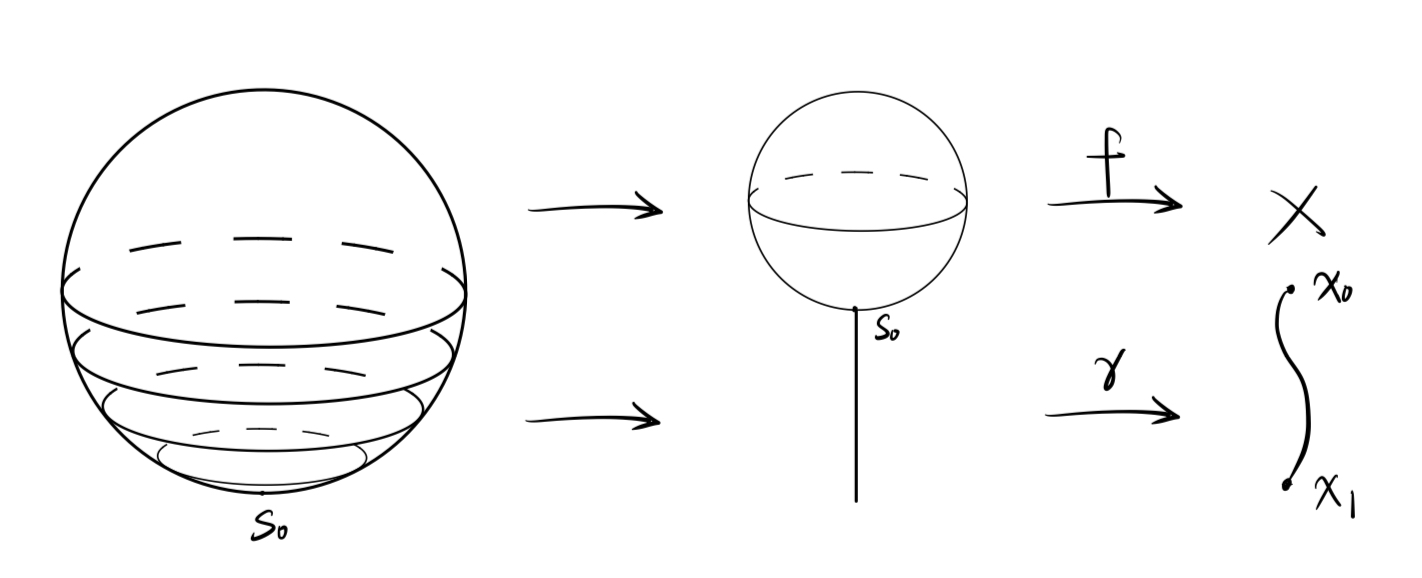
\includegraphics[width=300\unitlength]{./Figures/dependency-of-base-point.jpg}
    \end{center}
    One can check that $\gamma_*$ is an isomorphism with inverse 
    $\gamma_*^{-1} = \bar{\gamma}_*$. Moreover,
    \begin{equation*}
        \gamma\simeq\gamma'\;\mathrm{rel}\,\{0,1\}
        \Longrightarrow\gamma_*=\gamma'_*.
    \end{equation*}
    Especially when the path $\gamma$ starts and ends at the same point 
    $x_0$, that is, $\gamma$ is a loop at $x_0$, 
    we get a $\pi_1(X,x_0)$-action on $\pi_n(X,x_0)$ by:
    \begin{equation*}
        \gamma\cdot\alpha = \gamma_*(\alpha),\quad\gamma\in\pi_1(X,x_0),\;
        \alpha\in\pi_n(X,x_0).
    \end{equation*}
    Moreover, we have an equality
    \begin{equation*}
        \pi_n(X,x_0)\big/\pi_1(X,x_0)=[S^n,X].
    \end{equation*}
    When $\pi_1(X,x_0)$ acts on $\pi_n(X,x_0)$ trivially, 
    we say $X$ is $n$-simple. Under this assumption, 
    the isomorphism between $\pi_n(X,x_0)$ and 
    $\pi_n(X,x_1)$ is canonically defined. 
    Therefore we can use the notation $\pi_n(X)$ unambiguously.

    \begin{theorem}
        $\pi_n(X,x_0)\big/\pi_1(X,x_0)=[S^n,X].$
    \end{theorem}

    \begin{proof}
        In order to avoid ambiguity, we use $[\alpha]_n$, $[[\alpha]_n]_1$, 
        $[\alpha]$ to denote elements in $\pi_n(X,x_0)$, 
        $\pi_n(X,x_0)\big/\pi_1(X,x_0)$, $[S^n,X]$ respectively.

        The map between $\pi_n(X,x_0)\big/\pi_1(X,x_0)$ and $[S^n,X]$ is 
        naturally given, that is,
        \begin{align*}
            \phi:\pi_n(X,x_0)\big/\pi_1(X,x_0)&\to[S^n,X] \\
            [[\alpha]_n]_1&\mapsto[\alpha].
        \end{align*}

        $\phi$ is surjective: For any $[\alpha]\in[S^n,X]$, 
        let $x_1=\alpha(s_0)$. If $x_1 = x_0$, then
        \begin{equation*}
            \phi([[\alpha]_n]_1)=[\alpha].
        \end{equation*}
        If $x_1\neq x_0$, there is a path $\gamma$ from $x_0$ to $x_1$, then
        \begin{equation*}
            \phi([[\bar{\gamma}_*(\alpha)]_n]_1)=[\bar{\gamma}_*(\alpha)] = [\alpha].
        \end{equation*}

        $\phi$ is injective: If $[\alpha_0] = [\alpha_1]$, 
        where $\alpha_0,\alpha_1:(S^n,s_0)\to(X,x_0)$. 
        By definition of $[S^n,X]$, there is a homotopy
        \begin{equation*}
            H:S^n\times I\to X
        \end{equation*}
        satisfying $H(-,0)=\alpha_0(-),\,H(-,1) = \alpha_1(-)$. 
        We denote $\alpha_t(-) = H(-,t)$. Let
        \begin{equation*}
            \gamma(t):=H(s_0,t),\quad t\in I.
        \end{equation*}
        This defines a loop at $x_0$. Set
        \begin{equation*}
            \gamma_\tau(t)=\gamma(\tau+(1-\tau)t)=
        H(s_0,\tau+(1-\tau)t),\quad t\in I.
        \end{equation*}
        $\gamma_\tau$ is a path from $\gamma(\tau)$ to $\gamma(1) = s_0$. 
        Now we can give a homotopy between $\gamma_*(\alpha_0)$ and 
        $(c_{x_0})_*(\alpha_1)$ which fixes the base point:
        \begin{gather*}
            H':(S^n,s_0)\times I\to(X,x_0) \\
            H'(-,t)=(\gamma_t)_*(\alpha_t)(-).
        \end{gather*}
        Since $\alpha_t(s_0) = H(s_0,t)=\gamma(t) = \gamma_t(0)$, 
        the formula behind is well-defined. Moreover,
        \begin{gather*}
            H'(-,0)=\gamma_*(\alpha_0)(-),\\
            H'(-,1)=(c_{x_0})_*(\alpha_1)(-);\\
            H'(s_0,t)=(\gamma_t)_*(\alpha_t)(s_0)=x_0,\quad t\in I.
        \end{gather*}
        So $H'$ is what we need. Therefore
        \begin{equation*}
            \gamma_*([\alpha_0]_n)=[(c_{x_0})_*(\alpha_1)]_n=[\alpha_1]_n.
        \end{equation*}
        So that
        \begin{equation*}
            [[\alpha_0]_n]_1=[[\alpha_1]_n]_1.
        \end{equation*}

        \begin{center}
            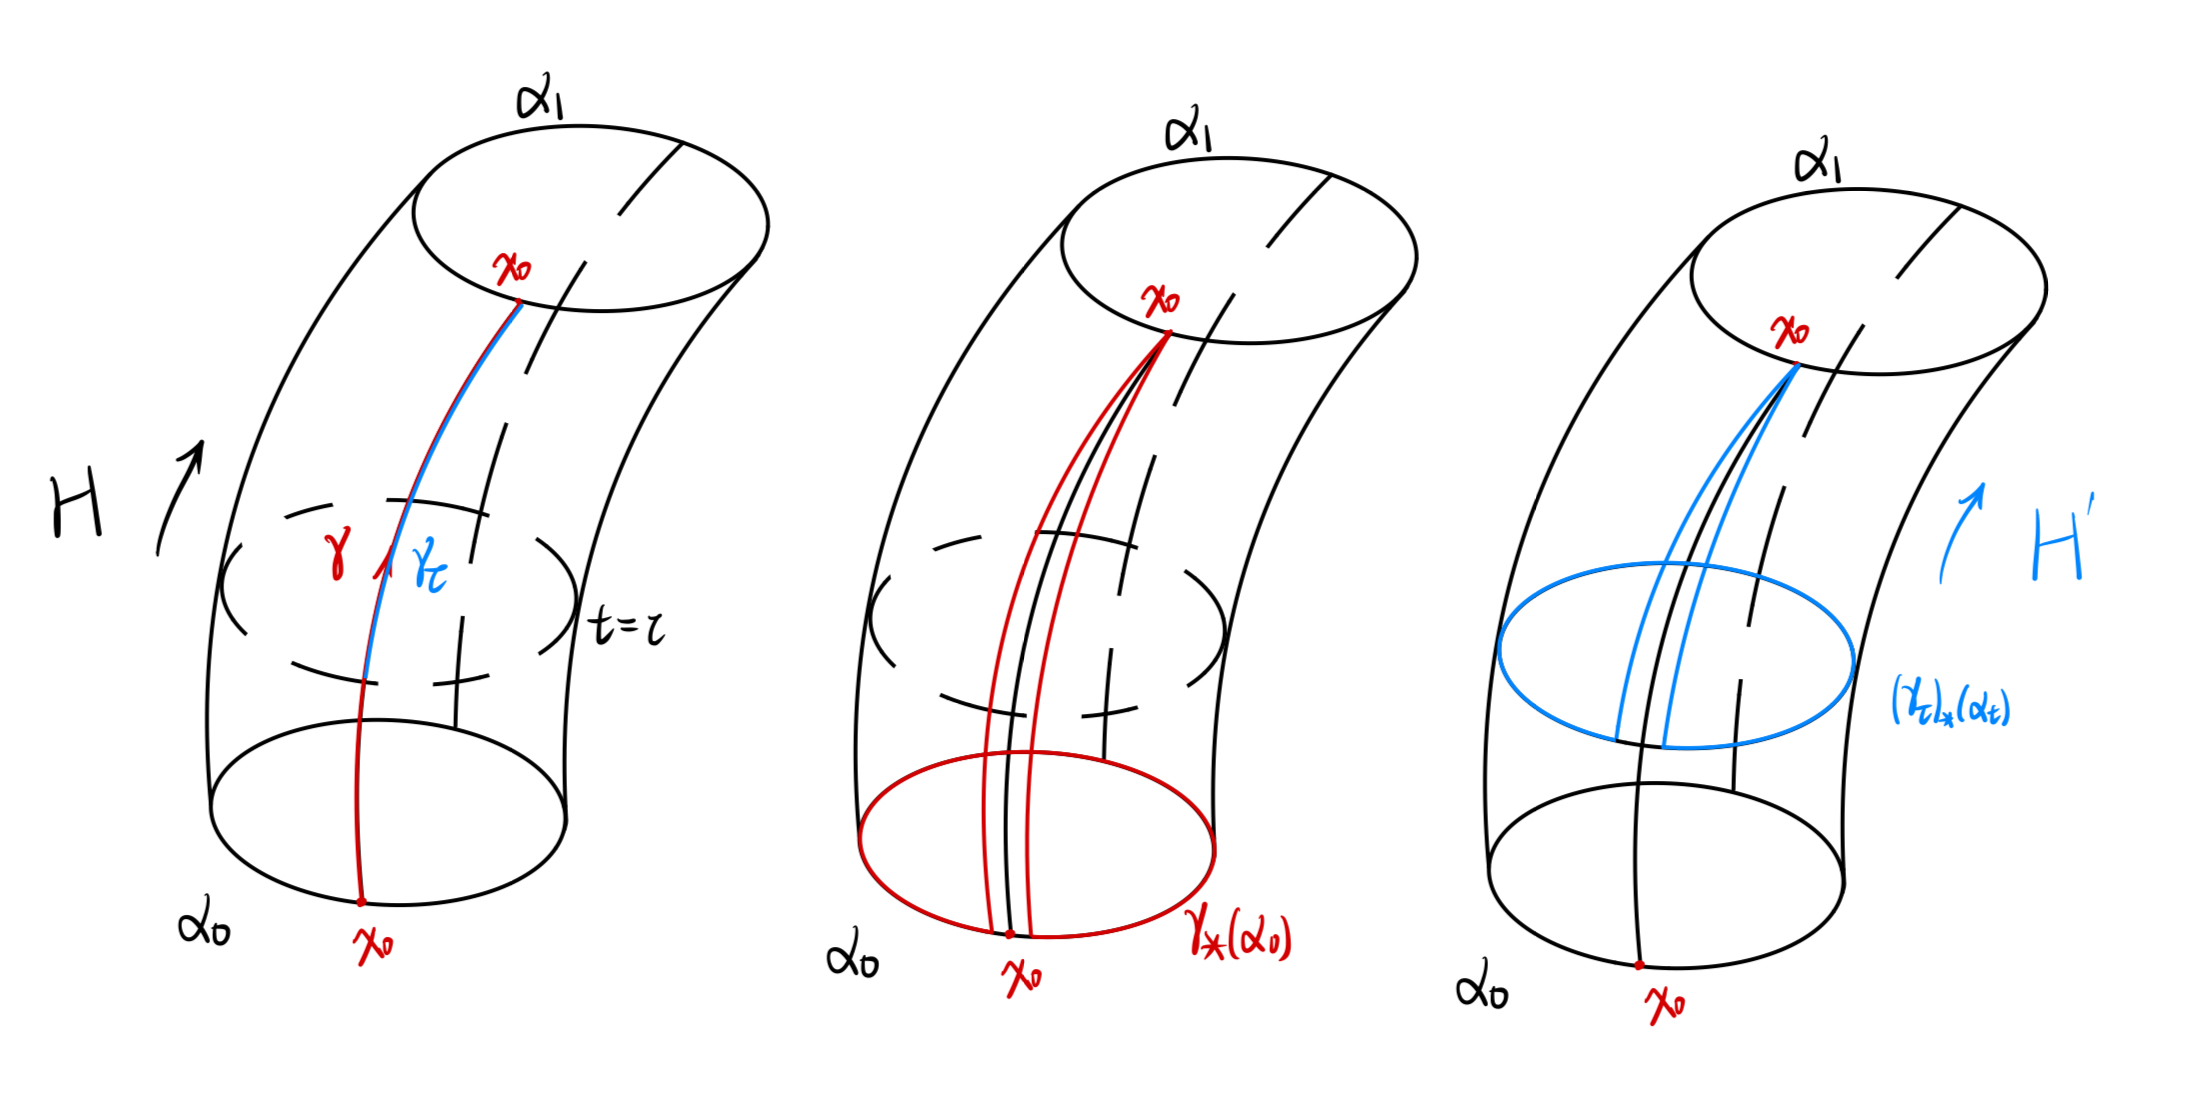
\includegraphics[width=350\unitlength]{./Figures/homotopy-to-relative-homotopy.jpg}
        \end{center}
    \end{proof}

    \subsection{Homotopy Lifting Property \& Homotopy Extending Property}
    \begin{proposition}[Homotopy Lifting Property]
        omit.
    \end{proposition}

    \begin{lemma}[Borsuk's Lemma]
        Any CW pair $(X,X')$ admits homotopy extending property.
    \end{lemma}

    \begin{proof}
        Suppose $X$ is a CW complex, $X'$ is its subcomplex and $f':X'\to Y$ can extend to $f:X\to Y$. For any homotopy $F':X'\times I\to Y$ with initial map $f'$, we extend it by induction.

        \textbf{Step 1:} For any vertex $x_0\in X^0 - X'$, we define
        \begin{equation*}
            F(x_0,t) = f(x_0), \quad t\in [0,1]
        \end{equation*}

        \textbf{Step 2:} Suppose we have extended the homotopy over the skeleton $X^n$. Now for any $(n+1)$-cell
        \begin{equation*}
            \psi:D^{n+1}\to X
        \end{equation*}
        The homotopy has been already defined on $S^n\times I$ and $D^{n+1}\times\{0\}$. To fill in the whole $D^{n+1}\times I$, we use the fact that there is a nice retraction (projection)
        \begin{equation*}
            r:D^{n+1}\times I\to(S^n\times I)\cup(D^{n+1}\times\{0\})
        \end{equation*}
        The following figure provides a nice illustration.
        \begin{center}
            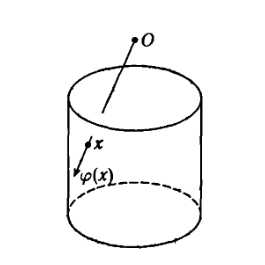
\includegraphics[width=200\unitlength]{./Figures/borsuk_lemma.png}
        \end{center}
        Thus we can extend the homotopy to any $(n+1)$-cell, so as $X^{n+1}$.
    \end{proof}

    \subsection{Exact Sequences for Fibrations}
    Given a fibration $p:E\to B$ with fibre $F$, we can derive an extremely useful long exact sequence of homotopy groups. First choose a base point $b_0\in B$, then choose $e_0\in p^{-1}(b_0)$. The fibering map $p$ induces a homomorphism
    \begin{equation*}
    p_*:\pi_n(E,e_0)\to\pi_n(B,b_0),\quad \forall\,n
    \end{equation*}
    Besides, the inclusion $i:F=p^{-1}(b_0)\hookrightarrow E$ induces
    \begin{equation*}
    i_*:\pi_n(F,e_0)\to\pi_n(E,e_0),\quad\forall\,n
    \end{equation*}
    The key is to construct a connecting homomorphism $\partial_*$.